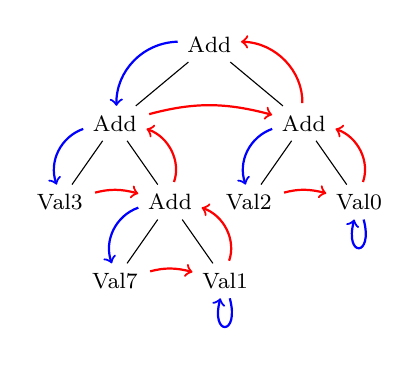
\begin{tikzpicture}
  \tikzstyle{every node}=[font=\footnotesize]
  \tikzstyle{level 1}=[level distance=10mm, sibling distance=24mm]
  \tikzstyle{level 2}=[level distance=10mm, sibling distance=14mm]
  \tikzstyle{level 3}=[level distance=10mm, sibling distance=14mm]
  \tikzstyle{load}=[->,thick,color=blue]
  \tikzstyle{unload}=[->,shorten <=1pt,thick,color=red]

  \node (root) {\AI{Add}}
  child {node (node1) {\AI{Add}} child {node (node2) {\AI{Val}\AS{}\AN{3}}} 
                                 child {node (node3) {\AI{Add}} 
                                   child {node (node4) {\AI{Val}\AS{}\AN{7}}}
                                   child {node (node5) {\AI{Val}\AS{}\AN{1}}}}} 
  child {node (node6) {\AI{Add}} child {node (node7) {\AI{Val}\AS{}\AN{2}}}
                                 child {node (node8) {\AI{Val}\AS{}\AN{0}}}};

  \draw[load] (root) to [ bend right=45] (node1);
  \draw[load] (node1) to [ bend right=45] (node2);
  \draw[unload] (node2) to [ bend left=15] (node3);
  \draw[load] (node3) to [ bend right=45] (node4);
  \draw[unload] (node4) to [ bend left=15] (node5);
  \draw[load] (node5) to [ loop below] (node5);
  \draw[unload] (node5) to [ bend right=45] (node3);
  \draw[unload] (node3) to [ bend right=45] (node1);
  \draw[unload] (node1) to [ bend left=15] (node6);
  \draw[load] (node6) to [ bend right=45] (node7);
  \draw[unload] (node7) to [ bend left=15] (node8);
  \draw[load] (node8) to [ loop below] (node8);
  \draw[unload] (node8) to [ bend right=45] (node6);
  \draw[unload] (node6) to [ bend right=45] (root);
\end{tikzpicture}
